\documentclass[12pt, a4paper]{article}
\usepackage{url,graphicx,tabularx,array,geometry}
\usepackage[utf8]{inputenc}
\usepackage{paralist}
\usepackage{latexsym}
\usepackage{fancyhdr}
\usepackage{ textcomp }
\usepackage{ mathrsfs }
\usepackage{amssymb}
\usepackage{hyperref}

\pagestyle{fancy}

\usepackage{amsmath}
\usepackage{amsfonts}
\usepackage{amssymb}

\DeclareUnicodeCharacter{00A0}{ }

\setlength{\parskip}{1ex} %--skip lines between paragraphs
\setlength{\parindent}{0pt} %--don't indent paragraphs

%-- Commands for header
\newcommand{\bs}{\ensuremath{\backslash}}
\renewcommand{\title}[1]{\textbf{#1}\\}
\renewcommand{\line}{\begin{tabularx}{\textwidth}{X>{\raggedleft}X}\hline\\\end{tabularx}\\[-0.5cm]}
\newcommand{\leftright}[2]{\begin{tabularx}{\textwidth}{X>{\raggedleft}X}#1%
& #2\\\end{tabularx}\\[-0.5cm]}
%\linespread{2} %-- Uncomment for Double Space
\begin{document}
\renewcommand{\headrulewidth}{0pt}
\fancyhf{}
\fancyhead[L]{
\leftright{\textbf{Zusammenfassung}}{Daniel Schmidt}
\line
\leftright{\textbf{Datenbanktheorie SS 16}}{}}
\fancyfoot[C]{\thepage}

\section*{Definition: Prädikatenlogische Sprache erster Stufe (PL1- Sprache)}
(ohne Funktionssymbole) \\
gegeben durch Paar $(A,F)$ mit 
\begin{itemize}
\item $A$ = Alphabet mit 
\begin{itemize}
\item unendlich viele Variable (aus einer Variablenmenge, genannt $Var_A$)
\item keine oder beliebig viele Konstantensymbole (aus einer Konstantenmenge Konst, genannt $Konst_A$)
\item mindestens ein Prädikatensymbol, möglicherweise unendlich viele Prädikatensymbole (aus einer Prädikatensymbolmenge, genannt $\textnormal{Präd}_A$)
\end{itemize}
\item $F$ = Menge aller wohlgeformten Formeln (Ausdrücke) mit Symbolen aus $A$
\end{itemize}

\section*{Definition: Term}
Ein Konstantensymbol aus $Konst_A$ oder eine Variable aus $Var_A$.

\section*{Definition: Atomare Formel (Atom)}
$p(t_1, \cdots, t_n)$ mit p ist n-stelliges Prädikatensymbol aus $A$ und $t_1, \cdots, t_n$ Terme

\section*{Satz: Konstruktionsregel für F}
kleinste Menge mit 
\begin{itemize}
\item Jedes Atom aus $A$ ist in $F$
\item Falls f und g in $F$ sind, dann sind auch $\lnot f, (f \wedge g), (f \vee g), (f \Rightarrow g), (f \Leftrightarrow g)$ in $F$
\item Falls X eine Variable ist und f in F, dann sind auch $(\forall X)(f)$ und $(\exists X)(f)$ in F
\end{itemize}

\section*{Definition: Interpretation}
Eine Interpretation I für eine PL1-Sprache $(A,F)$ ist ein Tripel (Dom, k, ext) mit:
\begin{itemize}
\item $dom$ ist eine nicht leere Menge, genannt Wertebereich (domain) von I
\item $k$ ist eine Abbildung von Konstantensymbolen aus $A$ in $dom$
\item $ext$ (extension) ist eine Abbildung von Prädikatensymbolen aus $A$ in Mengen von Tupeln, gebildet aus Werten von Dom unter Beachtung der Stelligkeit der Prädikatensymbole. Diese Tupelmengen heißen \textbf{Prädikate}, $ext(p)$ wird auch \textbf{Ausprägung} von p genannt.
\end{itemize}

\section*{Definition: Wahrheitswerte für PL1}
\paragraph{Konstanten und Variablen}
$\parallel t_1 \parallel_{I, \rho}: Var_A \cup Konst_A \rightarrow Dom$ definiert durch: 
\begin{itemize}
\item $k(c)$ für Konstantensymbole
\item $p(X)$ für Variablen
\end{itemize}

\paragraph{Relationen}
$\models_{I,\rho} p(t_1, \cdots, t_n)$ (Unter der Interpretation I und Belegung $\rho$ wahr) genau dann wenn $(\parallel t_1 \parallel_{I, \rho}, \cdots \parallel t_n \parallel_{I, \rho}) \in ext(\rho))$ für jedes Atom $p(t_1, \cdots, t_n)$ aus F

\section*{Definition: Folgerung ($F' \models f$)}
Formel $f \in F$ mit $F' \subseteq F$, falls jedes Modell von $F'$ auch ein Modell von $f$ ist.

\section*{Definition: unter Folgerbarkeit abgeschlossen}
Transitive Hülle von Folgerung

\section*{Definition: Theorie}
Besteht aus PL1-Sprache $(A, F)$ und Formelmenge $F' \subseteq F$, die unter Folgerbarkeit abgeschlossen ist. ($F'$: Sätze der Theorie)

\section*{Definition: Axiomatisierbar}
Theorie $T$, falls es eine entscheidbare Formelmenge $X \subseteq T$ gibt, derart dass alle Sätze von $T$ Folgerungen von $X$ (dann Axiomensystem von $T$ mit Elementen Axiome) sind

\section*{Satz: Modell einer Theorie}
Eine Interpretation I ist ein Modell einer Theorie $T$, falls I ein Modell der Menge aller Sätze von $T$  ist.

\section*{Definition: Konsistente Theorie}
Falls Theorie wenigstens ein Modell hat, sonst inkonsistent.

\section*{Definition: formale Ableitung}
Eine formale Ableitung einer Formel f von der Menge $\{f_1,..., f_m \}$ in der PL1- Logik ist eine Folge $b_1, \cdots, b_l$ von Formeln der Sprache $(A, F)$ mit 
\begin{itemize}
\item $b_l$ ist gleich f 
\item jede Formel $b_j, j \in \{ 1, \cdots l \}$ ist eine der Formeln $f_i, i \in \{ 1, \cdots, m \}$ oder eine allgemeingültige Formel, die aus $b_j$ in der Liste  vorangehender Formeln durch Anwendung einer Ableitungsregel der PL1-Logik erhalten werden kann.
\end{itemize}

\section*{Definition: ableitbar ($\vdash$)}
Falls es eine formale Ableitung gibt (aus $\emptyset$ oder Formelmenge)

\section*{Satz: Vollständigkeitssatz von Gödel}
\begin{align*}
&\emptyset \models f \Longrightarrow \vdash f
\end{align*}

\section*{Definition: Relationale Sprache}
$R = (A,F)$ mit 
\begin{itemize}
	\item Es gibt in A
	\begin{itemize}
		\item $1 \le |Konst_A| < \infty$
		\item $|\textnormal{Präd}_A| < \infty$
		\item ausgezeichnetes, zweistelliges Prädikatensymbol = (Gleichheit)
		\item ausgezeichnete Teilmenge einstelliger Prädikatensymbole, die \textbf{einfachen Typen}
	\end{itemize}
	\item Typen, kleinste Menge mit 
	\begin{itemize}
		\item jeder einfache Typ  von A ist ein Typ von R
		\item falls $\tau_1, \tau_2 \textnormal{ Typen von } R$, dann auch $(\tau_1 \wedge \tau_2), (\tau_1 \vee \tau_2), \lnot \tau_1$ Typen von $R$
	\end{itemize}
\end{itemize}

\section*{Definition: Relationale Interpretation}
Sei $R = (A, F)$ relationale Sprache, dann ist eine Interpretation $I = (Dom, k, ext)$ für R eine relationale Interpretation für R, wenn
\begin{itemize}
	\item k ist eine Bijektion (Dom ist endlich)
	\item $ext(=) = \{ (d,d) | d \in Dom \}$
\end{itemize}

\section*{Definition: Relationale Datenbank}
Tripel $(R, I, IB)$ mit
\begin{itemize}
	\item R ist eine relationale Sprache
	\item I ist eine relationale Interpretation
	\item IB ist eine Menge von Formeln von R, so dass insbesondere für jedes n- stellige Prädikatensymbol P, das verschieden ist von "=" und von den einfachen Typen, IB eine Formel der folgenden Gestalt enthalten muss ($\tau_1, \cdots \tau_n$ einfache Typen):
	\begin{align*}
	(\forall X_1) \cdots (\forall X_n) (p(X_1, \cdots X_n) \Rightarrow \tau_1(X_1) \wedge \cdots \wedge \tau_n(X_n))
	\end{align*}
\end{itemize}

\section*{Definition: Erlaubte relationale Datenbank}
Falls I ein Modell von IB ist

\section*{Definition: Intentionale, extentionale Prädikatensymbole}
\begin{itemize}
	\item Intentional: durch ein Programm definiert
	\item Extentional:  als Relationen in einer Datenbank gespeichert
\end{itemize}

\section*{Definition: Fixpunkttheorem (Knaster / Tarski)}
Sei $\tau$ eine monotone Transformation auf einem vollständigen Verband $(V, \le)$. Dann hat $\tau$ einen kleinsten Fixpunkt 
\begin{align*}
&lfp(\tau) = inf(\{ x \in V | \tau(x) le x \})
\end{align*}

\section*{Definition: Datalog Programm}
Ein Datalog-Programm P (ohne IBen(Integritätsbedingungen)) ist eine endliche Menge von Horn-Klauseln mit Jedes $d \in P$ ist entweder
\begin{itemize}
\item ein Fakt $q(...).$ ohne Variable
\item eine sichere Regel $q(...) :- p_1(...),...,p_n(...).$ mit $q\in iPraedikat$
\end{itemize}
Eine Regel heißt sicher, wenn alle in ihr vorkommenden Variablen beschränkt sind.


\section*{Definition: Bedeutung eines Datalog Programms}
Menge der Grundatome, die logisch aus P gefolgert werden können.


\section*{Satz von Gödel / Skolem}
Eine Klauselmenge P hat ein Modell genau dann wenn P hat ein Herbrand-Modell. Daraus folgt, dass ein Verfahren analog zu Wahrheitstabellen in der Aussagenlogik möglich ist.


\section*{Skolemisierung}
Jeder Formel der PL1 Logik, kann in eine erfüllbarkeitsäquivalte Formel in Skolem-Form gebracht werden. Dies bedeutet Pränexnormalform und alle Existenzquantoren durch Funktionen ersetzen.

\section*{Definition: Herbrand-Interpretation}
Eine Teilmenge der Herbrand- Basis

\section*{Grundatom}
Ein Grundatom f ist eine logische Folgerung einer Menge D von Datalog Klauseln (z.B. $D \vDash f$) $\diamondsuit_{Def}$. Jedes Herbrand Modell von D ist auch ein Modell von f.\\
Da f ein Grundatom ist gilt $D \vDash f \Longrightarrow f $ ist in jedem Herbrand-Modell von D enthalten. Das heißt $f \in \bigcap \{ I | I Herbrand-Modell von D \}$.\\
Sei $f \in \bigcap \{ I | I Herbrand-Modell von D \}$, dann ist f ein Grundatom und jedes Modell von D auch in Modell von f. 

\section*{Definition: Mege aller Konsequenzen}
$cons(D) =_{def} \{ f \in HB_D | D \vDash f \}$

\section*{Definition: Substitution}
Eine Substitution ist eine endliche Menge der Form
\begin{equation}
\{ X_1 / t_1, \cdots, X_n / t_n \}, X_1,...,X_n \text{ unterschiedliche Variablen, } t_1,....,t_n Terme, X_i \neq t_i
\end{equation}

Sei $\theta$ eine Substitution, t ein Term (Variable oder Konstante), so gilt \\

\begin{equation}
t\theta =_{def} \begin{cases} t_i, & \mbox{falls } t/t_i \in \theta \\ t, & \mbox{sonst} \end{cases}
\end{equation}

\section*{Definition: Grundsubstitution}
Substitution bei der alle $t_i$ Konstanten sind.

\section*{Definition: Unifizierbar}
Seien $L_1$ und $L_2$ heißen \textbf{unifizierbar}, wenn $(\exists \text{ Substitution } \Theta)(L_1\Theta = L_2\Theta)$. $\Theta$ heißt dann \textbf{Unifikator}.

\section*{Definition: Komposition}
Sei $\Theta = \{ X_1 / t_1, \cdots, X_n / t_n \}, \sigma = \{ Y_1 / n_1, \cdots, Y_m / t_m \}$ Substitutionen. \\
Die Komposition $\Theta\sigma$ von $\Theta$ und $\sigma$ erhält man aus 
\begin{equation}
X_1 / t_1\sigma, \cdots, X_m / t_m\sigma, Y_1 / n_q, \cdots, Y_m / n_m
\end{equation}
Durch Streichen von Elementen der Form Z/Z sowie $Y_i / n_i$ mit $Y_i = X_j$ für ein j$j \in \{1, ..., n\}$

\section*{Definition: allgemeinere Substitution}
Seien $\Theta, \varsigma$ Substitutionen, $\Theta$ heißt allgemeiner als $\varsigma \diamondsuit (\exists \text{Substitution} \delta)(\Theta \delta = \varsigma)$.
Seine $L_1, L_2$ Literale. Ein allgemeinster Unifikator (mgu) von $L_1 in L_2$ ist ein Unifikator von $L_1 und L_2$, der allgemeiner als alle anderen Unifikatoren ist.

\section*{Definition: Beweisbaum}
B entsteht aus S durch Anwendung von $\Theta$ auf alle Benennungen von Zielknoten. B repräsentiert einen Beweis für $g\Theta$, g benennung der Wurzel von S.

\section*{Definition: Tiefe eines Baums}
maximale Anzahl von Zielknoten auf einem Pfad von einem Blattknoten zur Wurzel. Entsprechend Knoten der Tiefe i, Ebene i eines Baumes. Zusätzlich: Spezielle Suchbäume (Tiefe 0) für Fakten aus P.

\section*{Suchbaum zu cons}
Sei P ein Datalog-Programm. Die Suchbaum  / Beweisbaum Methode, angewand auf alle Ziele $q(X_1, \cdots, X_{Stelligkeit(q)})$, q intentionales Prädikatesymbol von P, liefert cons(P) als Ergebnis

\section*{Suchbaum, Vollständigkeit}
Die Suchbaum / Beweisbaum Methode bleibt vollständig für ein Programm P, wenn nur Bäume mit max. Tiefe max\_fakt(P) betrachtet werden.

\section*{Resolutionsmethode}
Für allgemeine Klauselformen entwickelte Methode zum automatischen Beweisen.


\section*{Definition: Vollständiger Verband}
Partiell geordnete Mengt $(V, \le)$ bei der zu jeder Teilmenge ein Infinum($\bot_V$) \& Suprenum ($\top_V$)besteht.
Jeder endliche Verband (und jeder Teilmengenverband) ist vollständig.

\section*{Definition: Monotone Transformation}
Abbildung $\tau$ mit $(\forall a,b \in V) (a \le b \Rightarrow \tau(a) \le \tau(b))$.
 
\section*{Definition: Fixpunkt}
$a \in V: \tau(a) = a$

\section*{Satz: Fixpunkttheorem (Knaster / Tarski)}
Sei $\tau$ eine monotone Transformation auf einem vollständigen Verband $(V, \le)$. Dann hat $\tau$ einen kleinsten Fixpunkt 
\begin{align*}
&lfp(\tau) = inf(\{ x \in V | \tau(x) le x \})
\end{align*}

\section*{Magic Set Methode}
Transformiere ein Programm in eine Version, die für ein gegebenes Ziel die gleiche Ausgabe hat aber das Ziel bei bottom-up Auswertung berücksichtigt wird. \href{http://www.is.informatik.uni-kiel.de/~hjk/Datenbanktheorie/Magic_set.pdf}{Algorithmus}, \href{http://www.is.informatik.uni-kiel.de/~hjk/Datenbanktheorie/Magic_Beispiel.pdf}{Beispiel hier.}

\paragraph{Vorgehen}

\paragraph{1.Schritt}

Füge für das Ziel $g = q(\cdots)$ die Regel $query^{f\cdots}\footnote{Hochgestellte Zeichen sind Bindungsmuster (wie in Coral)}(X_1, \cdots, X_k) :- q^{\alpha}(\cdots).$ ein, wobei $X_1, \cdots, X_k$ Variablen aus $q^{\alpha}(\cdots)$ sind. Erzeuge für jede Regel $r \in P$ und jedes mögliche Bindungsmuster $\beta$ des Prädikates im Kopf von r eine Regel mit Bindungsmuster für jedes ihrer itensionalen Prädikate. Bestimme dabei unter Beachtung von $\beta$ für jedes Argument im Rumpf ob es ausgezeichnet ist oder nicht. Falls ein IDB-Pr¨adikat im Rumpf mehrfach auftritt, sollte man es durchnummerieren.

\paragraph{2.Schritt}

Forme $P^B_g$\footnote{Menge aller erreichbaren Regeln aus Schritt 1} zu $P^{magic}_g$\footnote{Bezüglich g äquivalent}. \\
Sei $P^{magic}_g := P^B_g$. Mach dann für jedes $r \in P^B_g$ und draus folgend für jedes Vorkommen $p^{\beta}\_i(t_1, \dots t_l)$ eines IDB-Prädikates im Rumpf von r folgendes:

\begin{itemize}
\item Streiche alle anderen Vorkommen von IDB-Prädikaten im Rumpf von r
\item Ersetze $p^{\beta}_g$ durch $magic\_r\_p^{\beta}\_i$
\item Streiche alle Variablen aus $(t_1, \dots t_l)$, die nicht ausgezeichnet sind. \footnote{Bei ``Prädikaten'' ohne Argumente die entsthen können: Fall entsprechende Relation $\neq \emptyset$ wahr, sonst falsch}
\item Streiche alle nicht ausgezeichneten EDB-Prädikate aus r.
\item Sei $z^{\alpha}(s_1, \cdots, s_k)$ das Prädikat im Kopf von r. Streiche alle Variablen aus $(s_1, \cdots, s_k)$, die nicht ausgezeichnet sind; $\alpha$ wird nicht verändert. \\
Ersetze $magic\_r\_p^{\beta}\_i(t_1, \dots t_l)$ durch $magic\_z^{\alpha}(s'_1, \cdots s'_{\widetilde{l}})\footnote{Änderungen aus letztem Schritt}$

\item Füge $P^{magic}_g$ die neuen Regeln hinzu
\end{itemize}
\paragraph{3. + 4.Schritt}
\newpage
\begin{figure}
\centering
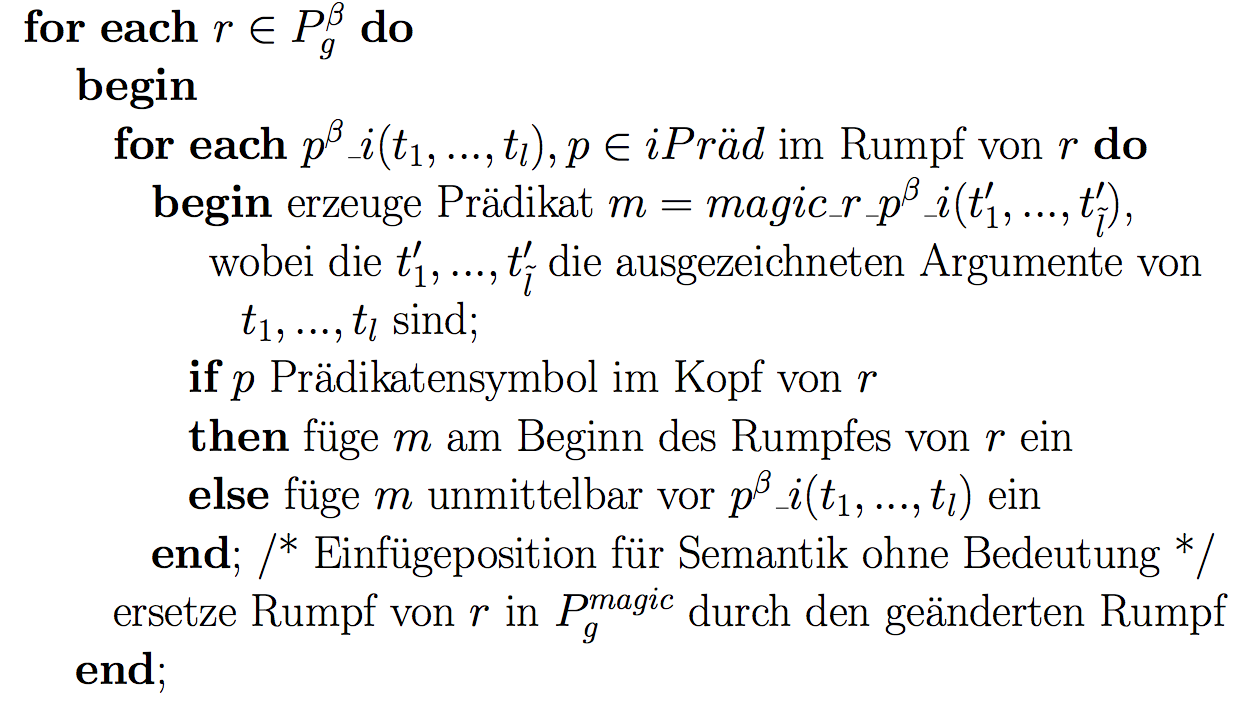
\includegraphics[width=0.95\linewidth]{img/img1}
\caption{}
\label{fig:img1}
\end{figure}

\begin{figure}
\centering
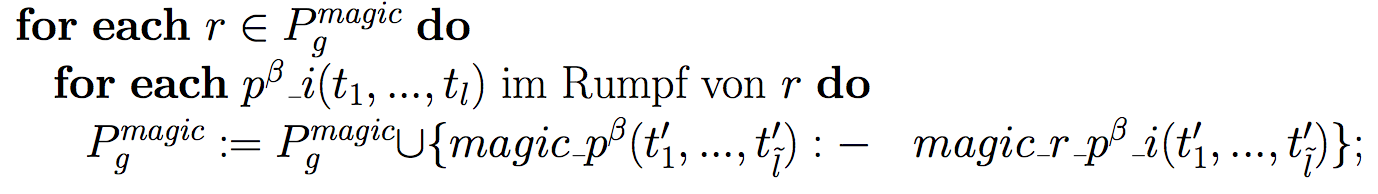
\includegraphics[width=0.95\linewidth]{img/img2}
\caption{}
\label{fig:img2}
\end{figure}

\section*{Definition: Ausgezeichnet}
\paragraph{Argument eines Teilziels}
Konstantensymbol, gemäß $\alpha$ gebunden, es in einem EDB-Prädikat auftritt, das ein ausgezeichnetes Argument hat.

\paragraph{EDB-Prädikat}
Alle seine Argumente sind ausgezeichnet

\section*{Definition: Abhängigkeitsgraph}
Gerichteter Graph $DG(P) = (V,E)$ eines Programms P, falls $V$ die Menge aller Prädikatensymbole von P und $e = (p,q) \in E \Leftrightarrow q$ kommt im Rumpf einer Regel von P vor, deren Kopfprädikat p ist. $e$ ist mit ``$\lnot$'' benannt, wenn q dabei wenigstens einmal negiert vorkommt.

\section*{Definition: Schichtung eines Programms}
Eine Folge $\Pi_1, \cdots, \Pi_n$ von Mengen von Prädikatensymbolen mit
\begin{itemize}
	\item $\{ \Pi_1, \cdots, \Pi_n \}$ ist eine Partition der Prädikatensymbole in P
	\item $q \in \Pi_i, r \in \Pi_j, (q,r)$ Kante in $DG(P) \Rightarrow i \ge j$, für alle Prädikatensymbole q,r aus P, $i,j \in \{1, \cdots, n\}$
	\item $q \in \Pi_i, r \in \Pi_j, (q,r)$ mit ``$\lnot$'' markierte Kante in $DG(P) \Rightarrow i > j$
\end{itemize}

\section*{Definition: Geschichtetes Programm}
Ein Programm P heißt geschichtet, wenn P eine Schichtung hat.

\section*{Satz: Schichtung / Zyklus}
Ein Programm P ist geschichtet, gdw. $DG(P)$ enthält keinen Zyklus mit einer Kante, die mit ``$\lnot$'' markiert ist.

\section*{Eigenschaften: Perfektes Modell}
``Kleinstes'' der minimalen Modelle, wenn das stärkste Gewicht darauf gelegt wird, dass die Prädikate niedriger Schichten klein bleiben

\section*{Satz: sicher geschichtet / perfektes Modell}
Sei P ein sicheres, geschichtetes Programm, dann ist das Perfekte Modell von P unabhängig von der Wahl der Schichtungen

\section*{Definition: Anfrage}
Sei $\sigma = \{ (RT_1, \alpha_1), \cdots, (RT_nm \alpha_n) \}$ ein relationales Datenbankschema über $\alpha = \bigcup^n_{i = 1} \alpha_i$ mit Wertebereichsfunktion dom. Sei $\alpha$ in eine genügend große Attributmenge $\alpha_0$ eingebettet\footnote{Enthalten darin}. \\
Eine Anfrage q auf $\sigma$ ist eine partielle Funktion
\begin{align*}
q | Z \sigma \Rightarrow R^{\infty}_{\beta}
\end{align*}

\section*{Definition: Anfragesprache}
Eine Anfragesprache zu $\sigma$ ist eine Menge $L_0$ von Ausdrücken zusammen mit einer Bedeutungsfunktion (in Zeichen: $(L_{\sigma}\footnote{Sprache}, \mu\footnote{Bedeutungsfunktion})$), so dass für jeden Ausdruck $e \in L_{\sigma}$ gilt: $\mu(e) \text{ ist eine Anfrage von } \sigma$ 

\section*{Definition: Ausdruckskraft}
Die Ausdruckskraft einer Anfragesprache $(L_{\sigma}, \mu)$ zu einer DB-Schema $\sigma$ ist definiert als $\mu(L_{\sigma}) =_{Def.} \{ \mu(e) | e \in L_{\sigma} \}$. Eine Sprache $(L_{\sigma}, \mu')$ ist \textbf{ausdrucksstärker} als eine Sprache $(L_{\sigma}, \mu)$, wenn gilt: $\mu(L_{\sigma}) \subseteq \mu'(L'_{\sigma})$
Im Fall $\mu(L_{\sigma}) = \mu'(L'_{\sigma})$ werden die Sprachen \textbf{äquivalent} genannt

\section*{Definition: Anfragesprache von $\rho$}
%TODO: Überprüfen wegen schlechter handschrift
Sei $\rho = \{ (RT_i, \alpha_i) | i \in Lm \}$ ein relationales Datenbankschema über $\alpha = \bigcup \alpha_i$ mit Werteberichsfunktion dom. Sei $\alpha$ in eine genügend große Attributmenge $\alpha_0$ eingebettet. Eine Anfrage q ist eine partielle Funktion mit $q: \delta_\rho \rightarrow R^{\infty}_\beta,  \delta \subseteq \alpha_0, R^{\infty}_\beta$ ist die Menge der verallgemeinerten DB-Relationen über $\beta$ (unendliche Teilmengen sind erlaubt). \\
Eine Anfragesprache zu $\rho$ ist eine Menge $L_\rho$ von Ausdrücken mit einer Bedeutungsfunktion $\mu$ (schreibe $(L_\rho, \mu)$), so dass für jeden Ausdruck $e \in L_\rho$ gilt $\mu(e)$ ist eine Anfrage an $\rho$.

\section*{Definition: Ausdruckskraft einer Anfragesprache von $\rho$}
Die Ausdruckskraft einer Anfragesprache $(L_\rho, \mu)$) zu $\rho$ ist definiert als $\mu(L_\rho) = \{ \mu(e) | e \in L_\rho \}$

\section*{Definition: Äquivalenz von Sprachen}
$(L'_\rho, \mu') = (L_\rho, \mu)$, wenn $\mu'(L'_\rho) = \mu(L_\rho)$. Kleiner und größer analog.
Falls Anfragesprache L für alle $\rho$ äquivalent zu Anfragesprache L' ist werden beide als äquivalent bezeichnet.

\section*{Satz 2.1}
Sei e ein zu einem gegebenen Datenbankschema $\rho$ passender RA-Ausdruck ohne Komplement. Dann gibt es einen äquivalenten zu e passenden Ausdruck der RA e' in dem als Operatoren nur Selektionen mit einfachen Vergleichsausdrücken, direktes Produkt, Projektion, Umbenennung, Differenz, Vereinigung vorkommen. Als Operanden ermittelt e' neben Relationstypbezeichnern aus $\rho$ nur (extensionale) DB-Relationen der Form $\{(A, C), A \in \alpha_\rho, c \in dom(A) \} $\\

Weitere Einschränkungen sind möglich $\rightarrow$ Projektionen nur auf ein Attribut, Vergleichsausdrücke = und >. \\
Falls Komplementbildung hinzugenommen, Differenz nicht mehr notwendig: \\
$R \backslash S = (R[kompl] \cup S)[kompl]$

\section*{Satz 2.2}
%TODO: Überprüfen wegen schlechter handschrift
Eine derart ??? Operationsmenge der RA ist minimal, d.h. es kann keine Operation entfernt werden, ohne dass die Ausdruckskraft eingeschränkt ist.

\section*{Satz 2.3}
Sei RT der Bezeichner eines beliebigen, zweistelligen Relationstyp über abzählbaren unendlichen Wertebereich. Sei Rt* der Relationstyp für die transitive Hülle von Relationen des Typs RT. Es gibt keinen Ausdruck  der Relationenalgebra mit der Eigenschaft $e(RT) ? = RT*$. \\

Gegeben Wertebereich $\{a_1, a_2, \cdots \}$ ohne Ordnungsrelation. Betrachte $R_l = \{ (a_i, a_i+1) | i \in [l-1] \}$ für $l \in \mathbb{N} \}$. $R_l$ ist eine mathematische Relation, die Tupel sind also geordnet. Zeige $e(R_l) \neq R*_l$ für jeden RA - Ausdruck e, der zu Wertebereichen passt und für genügend großes l. $e(R_l)$ bedeutet $R_l$ für RT eingesetzt. RA-Operationen sind anzupassen (wir haben keine Bezeichner $\leadsto$ Permutationen einführen) .
\begin{itemize}
	\item Projektion: \footnote{entspricht $\exists$: es gibt da was in der spalte, aber was das ist, ist mir egal} erlaubte Permutationen (vgl p(x) :- r(y,x) ist Projektion in r)
	\item Selektionen mit atomaren Vergleichsausdrücken der Form $i = a_m, i \neq a_m, i = j, i \neq j$ für $i,j \in [k], m \in [l]$ k ist bestimmt durch Größe der konstruierten Tupel $(b_1, \cdots, b_k), b_i \in \{a_1, \cdots a_l \}$
\end{itemize}

\section*{Lemma 2.1} 
Sei e ein beliebiger RA-Ausdruck, der zum Wertebereich $\{ a_1, a_2, a_3, \cdots \}$ passt und zu RT. Dann lässt sich $e(R_l)$ für ein genügend großes l darstellen als
\begin{align*}
&e(R_l) = \{ (X_1, \cdots, X_K) / \Psi(X_1, \cdots, X_K) \} \subseteq \{ a_1, \cdots, a_l \}^K
\end{align*}

mit $K \in \mathbb{N}$, $\Psi$ aussagenlogischer Ausdruck in disjunktiver Form, wobei atomare Ausdrücke nur Vergleichsausdrücke der oben genannten Form auftreten.


\section*{Definition: Vollständigkeit einer Anfragesprache}

Eine Anfragesprache $(L_0, \mu)$ zu einem DB-Schema $\sigma$ heißt vollständig, wenn gilt: 
\begin{enumerate}
\item Für jeden Ausdruck $e \in L_\sigma$ ist $\mu(e)$ berechenbar und generisch
\item Für jede berechenbare und generische Anfrage q an $\sigma$ gibt es einen Ausdruck $e \in L_\sigma$ mit $\mu(e) = q$.
\end{enumerate}


\section*{Definition: Abgeschlossenheit einer Anfragesprache}

Eine allgemeine Anfragesprache L mit Interpretationsvorschrift $\mu$ heißt abgeschlossen, wenn sie zu jedem Datenbank-Schema $\sigma$ eine vollständige Anfragesprache $(L_\sigma, \mu)$ enthält.
Offensichtlich: 
\begin{itemize}
\item Alle RA-Anfragen sind berechenbar und generisch
\item Die RA ist nicht abgeschlossen (s. Satz 2.3)
\end{itemize}

\end{document}
